\documentclass[xcolor=table,final]{beamer} %,handout
\usepackage{etex}

\usepackage{amsfonts,amssymb}
\usepackage{url}
%% \usepackage{hyperref}

\usepackage[T2A]{fontenc}
\usepackage[utf8]{inputenc}
\usepackage[english]{babel}
\usepackage[linesnumbered,vlined]{algorithm2e}
\usepackage{booktabs}
\usepackage{fancybox}
\usepackage{blockmatrgraph}

\usepackage{tikz}
\usetikzlibrary{matrix,shadows,arrows,shapes,patterns,trees}
\usepackage{dirtree}

\usepackage{ulem}

\newcommand{\Bsof}{\texttt{BSOF}\xspace}
\newcommand{\Bstri}{\texttt{BSTRI}\xspace}
\newcommand{\Bsoftri}{\texttt{BSOFTRI}\xspace}
\newcommand{\Bsoi}{\texttt{BSOI}\xspace}
\newcommand{\Gemm}{\texttt{DGEMM}\xspace}
\newcommand{\Trmm}{\texttt{DTRMM}\xspace}
\newcommand{\Trsm}{\texttt{DTRSM}\xspace}
\newcommand{\Lacpy}{\texttt{DLACPY}\xspace}
\newcommand{\Trtri}{\texttt{DTRTRI}\xspace}
\newcommand{\Geqrf}{\texttt{DGEQRF}\xspace}
\newcommand{\Orgqr}{\texttt{DORGQR}\xspace}
\newcommand{\Ormqr}{\texttt{DORMQR}\xspace}
\newcommand{\Ilaenv}{\texttt{ILAENV}\xspace}

\mode<presentation>{
  \hypersetup{pdfpagemode=FullScreen}
  
  %% \usetheme{Berkeley}
  %% \usecolortheme{crane}%{seagull}
  %% \usetheme{AnnArbor}
  \usecolortheme{rose}

  \setbeamercovered{transparent}
}

\mode<handout>{
  \useinnertheme{default}
  \useoutertheme{infolines}
  \usecolortheme{default}
  \usefonttheme{professionalfonts}

  \usepackage{pgfpages}
  \pgfpagesuselayout{2 on 1}[a4paper,border shrink=4mm]

  \setbeamercolor{structure}{fg=black}
  \setbeamerfont{structure}{series=\bfseries} 
}

\title[BSOI on Multicores with GPUs]{%
  Structured Orthogonal Inversion of Block $p$-Cyclic Matrices 
  on Multicores with GPU Accelerators}
\subject{GPU and Accelerator Computing}


\author[Z.\,Bai]{
  Sergiy Gogolenko\inst{1} 
  \and \alert{Zhaojun Bai}\inst{2}
  \and Richard Scalettar\inst{2}
}

\institute[UC Davis]{%
  
\includegraphics[height=2cm]{./figs/logo/donntu-logo.png}%Donetsk National Technical University
  \hspace*{0.75cm}~%
  
\includegraphics[height=2cm]{./figs/logo/ucdavis-logo.png}%University of California, Davis
}
%% \titlegraphic{
\includegraphics[width=4cm]{./figs/logo/ucdavis-logo.png}}

\date[Euro-Par 2014] {%
  Euro-Par 2014\\%
  \footnotesize{Porto, Portugal}\\%
  \footnotesize{August 25-29}
}


\pgfdeclareimage[height=1.2cm]{university-logo}{./figs/logo/ucdavis-logo.png}

\begin{document}

\frame[plain]{\titlepage}

\begin{frame}{Outline}%[pausesections]{Outline}
  \tableofcontents
\end{frame}

\section{Background \& motivation}

%% \subsection{Problem formulation}

\begin{frame}{Problem formulation}
  \begin{definition}[$p$-cyclic matrix]
    \begin{equation} \label{eq:matr_A}
      H =
      \begin{bmatrix}
        A_1 &    &    &  & B_p   \\
        B_1 & A_2 &    &  &  \\
        & B_2 & A_3 &  &     \\
        &        & \ddots & \ddots &         \\
        &     &          & B_{p-1} & A_p
      \end{bmatrix}
      ,
    \end{equation}
    where $A_i$ and $B_i$ are non-zero blocks
  \end{definition}
\end{frame}

\begin{frame}{Applications}{Major application areas}
  %% \structure{Major application areas}
  \begin{itemize}
  \item numerical solving differential equations
    \begin{itemize}
    \item two-point BVPs: \\
      {\footnotesize
        multiple shooting \\
        and finite difference schemes
      }
    \item various IBVPs: \\
      {\footnotesize
        orthogonal spline collocation methods (including elliptic BVPs), \\
        method of lines,\\
        and Keller's box scheme
      }
    \end{itemize}
  \item Markov chain modeling
    \begin{itemize}
    \item periodic transition graphs for queuing networks
    \item stochastic Petri nets
    \end{itemize}
  \item quantum Monte Carlo (QMC) simulations 
    %of Hubbard models for strongly correlated materials
  \end{itemize}

  \pause
  \begin{exampleblock}{%% Inevitable
      Key numerical kernels}
      \begin{itemize}
      \item solving linear systems
      \item explicite \alert{inversion}
      \end{itemize}
      %% \begin{center}
      %% \end{center}
  \end{exampleblock}

\end{frame}

\begin{frame}{Applications}{Case study: %
    %% Study thermodynamics, kinetics and magnetic properties with
    2D and 3D time-dependent determinant QMC}
  %% \begin{block}{Objective}
  %%   Study thermodynamics, kinetics and magnetic properties of meterials
  %% \end{block}
  \begin{block}{Hubbard model}
    \begin{columns}
      \begin{column}{0.35\textwidth}
        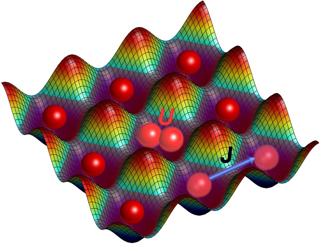
\includegraphics[width=1.\textwidth]{figs/extras/hubbard_model}
      \end{column}
      \begin{column}{0.7\textwidth}
        \begin{equation*}
          \footnotesize
          \begin{split}
            {\cal H} =& 
            \overbrace{
              -t \sum_{\langle i,j \rangle,\sigma} 
              (c^{\dagger}_{i,\sigma} c^{}_{j,\sigma}+ c^{\dagger}_{j,\sigma}c^{}_{i,\sigma})%
            }^{\text{$J$ -- kinetic energy (tunneling)}} - 
            \\ -&
            \underbrace{
              \underbrace{
                \mu \sum_{i=1}^{N} (n_{i\uparrow} + n_{i\downarrow})%
              }_{\text{chemical energy}} +
              \underbrace{
                U \sum_{i=1}^{N} (n_{i\uparrow} -\frac{1}{2}) (n_{i\downarrow}-\frac{1}{2})%
              }_{\text{potential energy}}
            }_{\text{$U$ -- on-site interaction}},
          \end{split}
        \end{equation*}
      \end{column}
    \end{columns}
  \end{block}
  \pause
  \begin{enumerate}
  \item 
    \alert{Spatial and temporal discretization} of partition function $\cal Z$
    for interacting ``Hubbard particles''
    %% Trotter-Suzuki decomposition
    %% Hubbard-Stratonovich (HS) transformation
    results in \alert{$p$-cyclic matrices} with identity diagonal blocks 
    \alert{$\cal M$} (Hubbard matrices)
  \item 
    \alert{inverse of $\cal M$} (Green’s function)
    must be computed \alert{at each iteration} of DQMC
    and is essential to express physical observables
  \end{enumerate} 
\end{frame}

\section{Algorithm}

\subsection{Serial BSOI algorithm}

\begin{frame}{Basic algorithms}{Framework}
  \begin{block}{Factorization-based approaches to matrix inversion}
    \begin{itemize}
    \item based on Gaussian elimination
      \begin{itemize}
      \item row partial pivoting is fast but unstable for $p$-cyclic matrices (S. Wright, 1993)
        %% \item panel rank-revealing pivoting strategy is stability in most cases but does not preserve structure
      \end{itemize}
    \item based on structured orthogonal factorization
      \begin{itemize}
      \item factorization is stable and has 
        identical complexity to the best known Gaussian elimination algorithms
      \end{itemize}
    \end{itemize}
  \end{block}

  \pause
  \begin{block}{Orthogonal inversion approach}
    \begin{centering}
      $\structure{\fbox{$H^{-1} = R^{-1}Q^T$}}$
    \end{centering}
    \begin{enumerate}
    \item Compute QR decomposition $H = QR$
    \item Invert the factor $R$ 
    \item Apply the factor $Q$ to $R^{-1}$ 
    \end{enumerate}
  \end{block}
\end{frame}

\begin{frame}{Basic algorithms}{Structured orthogonal factorization}
  \begin{block}{{\tt BSOF} -- Wright's serial version of SOF algorithm}
    \begin{algorithm}[H]%[thb]
      \KwData{$H$, $n$, $p$}
      \KwResult{$R$, $\{Q^{(k)} | 1 \leq k < p - 1 \}$}
      \BlankLine

      $R \gets O$; $\tilde{A}_1 \gets A_1$ ; $\tilde{B}_1 \gets B_p$\; 

      \For{$k \in \{1, 2,..., p-2 \}$ }{
        Compute regular QR: 
        $Q^{(k)} 
        \begin{bmatrix}
          R_{kk} \\ 0
        \end{bmatrix}
        =
        \begin{bmatrix}
          \tilde{A}_k \\ B_k
        \end{bmatrix}$\;

        %% Update 
        $\begin{bmatrix}
          R_{k,k+1} & R_{k,p} \\ \tilde{A}_{k + 1} & \tilde{B}_{k + 1}
        \end{bmatrix}
        \gets
        \left( Q^{(k)} \right)^{T} 
        \begin{bmatrix}
          0 & \tilde{B}_k \\ {A}_{k + 1} & 0
        \end{bmatrix}$;
      }
      
      Compute the QR: 
      $Q^{(p-1)} 
      \begin{bmatrix}
        R_{p-1,p-1} & R_{p-1,p}\\
        0 & R_{p,p}
      \end{bmatrix}
      = \begin{bmatrix}
        \tilde{A}_{p-1} & \tilde{B}_{p-1}\\ 
              {B}_{p-1} & {A}_{p,p}\\ 
      \end{bmatrix}$;
    \end{algorithm}
  \end{block}
\end{frame}


\begin{frame}{Basic algorithms}{Structured orthogonal factorization: Result}
  \tikzstyle{every picture}+=[remember picture]

  \tikzstyle{matrix node}   = [drop shadow,anchor=base]
  \tikzstyle{input matrix}  = [draw=red!50!black!50,fill=red!20,matrix node]
  \tikzstyle{result matrix} = [draw=green!50!black!50,fill=green!20,minimum height=7em,matrix node]
  \tikzstyle{data arrow}    = [->,line width=1pt,draw=red]
  \tikzstyle{input arrow}   = [data arrow,draw=red!50!black!50]
  \tikzstyle{result arrow}  = [data arrow,draw=green!50!black!50]

  \begin{equation*} \label{eq:matr_H}
    \tikz[baseline]{\node[input matrix] (matrH) {$\displaystyle
        \begin{bmatrix}
          A_1 &    &    &  & B_p   \\
          B_1 & A_2 &    &  &  \\
          & B_2 & A_3 &  &     \\
          &        & \ddots & \ddots &         \\
          &     &          & B_{p-1} & A_p
        \end{bmatrix}
        $};}
  \end{equation*}

  \pause

  \begin{center}
    \tikz[baseline]{\node%% [ellipse,drop shadow,fill=white,draw]
      (signQR) {{\tt BSOF} algorithm};}
  \end{center}

  \begin{equation*} \label{eq:matr_H_decomposition}
    \tikz[baseline]{\node[result matrix] (matrQ) {$\displaystyle
        \prod_{k=1}^{p-1}
        %% \begin{bmatrix}
        %%   I_{n(k-1)} &  &  &  &  \\
        %%   &  & Q_{11}^{(k)} & Q_{22}^{(k)} &  \\
        %%   &  & Q_{21}^{(k)} & Q_{22}^{(k)} &  \\
        %%   &  &  &  & I_{n(p-k-1)}
        %% \end{bmatrix}
        \begin{bmatrix}
          I_{n(k-1)}  &  &  &  \\
          &  & Q_{1:2,1:2}^{(k)} &  \\
          &  &  & I_{n(p-k-1)}
        \end{bmatrix}
        $};}
    \times
    \tikz[baseline]{\node[result matrix] (matrR) {$\displaystyle
        \begin{bmatrix}
          R_{11} & R_{12} &  & R_{1,p} \\
          & \ddots & \ddots & \vdots \\
          &        & R_{p-1,p-1} & R_{p-1,p}  \\ 
          &        &           & R_{p,p}
        \end{bmatrix}
        $};}
  \end{equation*}

  \begin{tikzpicture}[overlay]
    %% \path[->] (matrH.south west) edge [bend right] (matrQ);
    %% \path[->] (matrH.south east) edge [bend left] (matrR);
    \draw[input arrow]  (matrH.south) -- (signQR);
    \draw[result arrow] (signQR.west) edge [bend right] (matrQ.north);
    \draw[result arrow] (signQR.east) edge [bend left] (matrR.north);
  \end{tikzpicture}
\end{frame}

\begin{frame}{Basic algorithms}{Inversion via block back substitution}
  \begin{block}{{\tt BSTRI\_RV} -- Row Version of the BBS}
    \begin{algorithm}[H]
      \SetKwFunction{Batched}{Batched}

      \KwData{$R$, $n$, $p$}
      \KwResult{$X$}
      \BlankLine

      $X \gets O$\; 
      $X_{p-2:p,p-2:p}\gets R_{p-2:p,p-2:p}^{-1}$\;
      \Batched$_{i = 1:p-3}$ \{$X_{ii}\gets R_{ii}^{-1}$\} \;
      $X_{1:p-3,p}\gets R_{1:p-3,p} X_{p,p} $ \;
      \Batched$_{i = 1:p-3}$ \{$X_{i,p}\gets -X_{ii}  R_{i,p}$, $X_{i,i+1}\gets -X_{ii}  R_{i,i+1}$ \} \;
      \For{$i \in \{p-3, p-4,..., 1 \}$ }{ 
        $X_{i,i+2:p} \gets X_{i,i+2:p} + X_{i,i+1} X_{i+1,i+2:p} $ \;  
        $X_{i,i+1} \gets X_{i,i+1}  X_{i+1,i+1}$\;}
    \end{algorithm}    
  \end{block}
  
  \begin{block}{{\tt BSTRI\_CV} -- Column Version of the BBS}
    Similar to {\tt BSTRI\_RV}
  \end{block}
\end{frame}

%% \begin{frame}{Basic algorithms}{}
%% \end{frame}

\begin{frame}{Basic algorithms}{%
    Applying the orthogonal factors (Householder reflectors) to $R^{-1}$}
  \begin{block}{{\tt BSOI} -- Update $X$ via applying $Q^{T}$}
    \begin{algorithm}[H]
      \KwData{$X$, $\{Q^{(k)} | 1 \leq k < p - 1 \}$, $n$, $p$}
      \KwResult{$X$}
      \BlankLine

      \For{$k \in \{p-1, p-2,..., 1 \}$}{
        $X_{1:p,k:k+1} \gets X_{1:p,k:k+1} Q^{(k)T} $
        %\label{alg:apply_Qk_in_total}
      }
      \BlankLine
    \end{algorithm}    
  \end{block}

  \begin{block}{{\tt BSOI\_Qk} -- Applying $Q_k^{T}$}
    \begin{algorithm}[H]
      \KwData{$X_{1:p,k:k+1}$, $Q^{(k)}$, $n$, $p$}
      \KwResult{$X_{1:p,k:k+1}$}

      $W_{1:k+1,k:k+1} \gets X_{1:k+1,k:k+1} Q^{(k)T} $\;
      % $X_{1:k+1,k:k+1} \gets W$\;
      $W_{k+2:p,k:k+1} \gets X_{k+2:p,k:k+1} Q_{1:2,2}^{(k)T}$\;
      $X_{1:p,k:k+1} \gets W$;
    \end{algorithm}    
  \end{block}
\end{frame}

\begin{frame}{Basic algorithms}{Complexity}  
  \begin{block}{Operation counts}
    \begin{center}
      \rowcolors[]{1}{blue!20}{blue!10} %\rowcolors{1}{Blue!20}{Blue!5}
      \begin{tabular}{r|l|c|c|c}
        \toprule
        Phase & Routine & Additions & Multiplications & Total Flops  \\
        \hline
        I&{\tt BSOF} & 
        $\displaystyle\Theta\left(\frac{23}{3} n^{3} p\right)$
        & $\displaystyle\Theta\left(\frac{23}{3} n^{3} p\right)$
        & $\displaystyle\Theta\left(\frac{46}{3} n^{3} p\right)$\\
        II&{\tt BSTRI\_RV} & 
        $\displaystyle\Theta\left(\frac{1}{2} n^3 p^{2}\right)$
        & $\displaystyle\Theta\left(\frac{1}{2} n^3 p^{2}\right)$
        & $\displaystyle\Theta\left(n^3 p^{2}\right)$\\
        \cline{2-5}
        &{\tt BSTRI\_CV} & 
        $\displaystyle\Theta\left(n^3 p^{2}\right)$
        & $\displaystyle\Theta \left(n^3 p^{2}\right)$
        & $\displaystyle\Theta \left(2 n^3 p^{2}\right)$\\
        III&{\tt BSOI} & 
        $\displaystyle\Theta \left(3 n^3 p^2\right)$
        & $\displaystyle\Theta \left(3 n^3 p^2\right)$
        & $\displaystyle\Theta \left(6 n^3 p^2\right)$\\
        \bottomrule  
      \end{tabular}
    \end{center}
    \pause
    To sum up, 
    \[
    \fbox{
      $\text{Total complexity} = \alert{\displaystyle\Theta\left(\frac{7}{2} n  N^2\right)}$}
    \]
  \end{block}
\end{frame}

\subsection{Parallel ``host-device'' BSOFI}

\begin{frame}{Parallel ``host-device'' BSOFI}{Framework}
  \resizebox{.75\width}{.75\height}{
    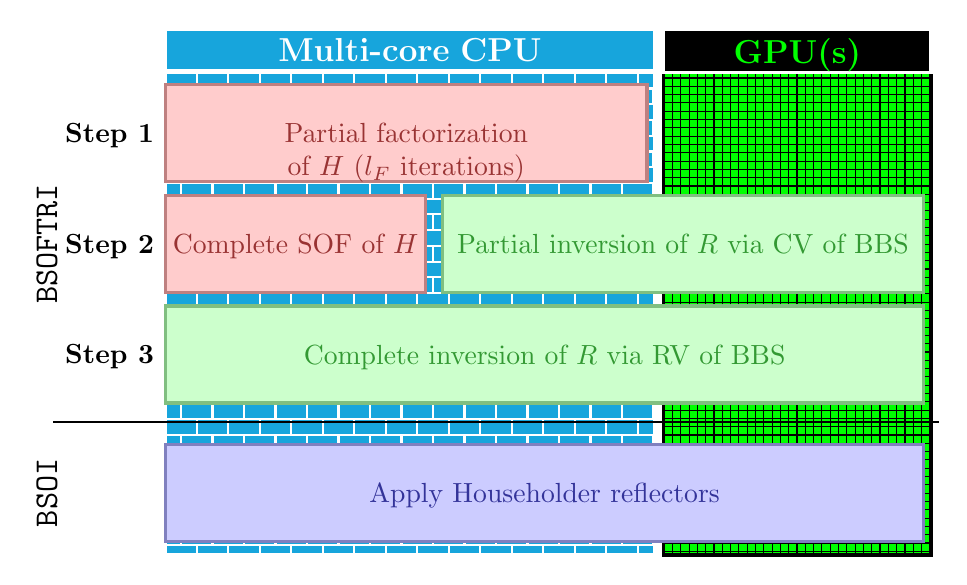
\begin{tikzpicture}[>=latex,text depth=0.0ex]
  \tikzstyle{algBlockStyle}  = [rectangle,very thick,inner sep=2pt,minimum height=3.5em,draw,anchor=north west,text centered]
  %\tikzstyle{algBlockStyle}  = [fill=red!50!black!50,draw=none,text=white,shading angle=0,inner color=white,outer color=red!50!black!80]
  \tikzstyle{blockBSOF}  = [draw=red!50!black!50,fill=red!20,text=red!50!black!80]
  \tikzstyle{blockBSTRI} = [draw=green!50!black!50,fill=green!20,text=green!50!black!80]
  \tikzstyle{blockBSOI}  = [draw=blue!50!black!50,fill=blue!20,text=blue!50!black!80]

  %\tikzstyle{frameGPU}  = [anchor=north west,very thin,preaction={fill, black},pattern=dots,pattern color=green,draw]
  \tikzstyle{frameGPU}  = [anchor=north west,very thick,preaction={fill, green},pattern=grid,pattern color=black,draw]
  \tikzstyle{frameCPU}  = [anchor=north west,very thick,preaction={fill,cyan!90!black!100},pattern=bricks,pattern color=white,draw=white]
  

%below of=1, xshift=-1.5cm, very thin,shading=true,inner color=white,outer color=blue!40

  \node[frameCPU,text width=17em,minimum height=19em] at (0,2em) {};
  \node[fill=cyan!90!black!100,text=white,font=\bfseries,text width=17em,anchor=north west,text centered,very thick,draw=white] at (0,2em) {\large Multi-core CPU};
  \node[frameGPU, text width=9em,minimum height=19em] at (18em,2em) {};
  \node[fill=black,text=green,font=\bfseries,text width=9em,anchor=north west,text centered,very thick,draw=white] at (18em,2em) {\large GPU(s)};
  % . 
  \node[algBlockStyle,blockBSOF,text width=17em] (BSOFTRI1) {%
    Partial factorization of $H$ ($l_F$ iterations)
    % (without updating the last block column)
  };
  \node [anchor=east] at (BSOFTRI1.west) {{\bf Step 1}};

  \node[algBlockStyle,blockBSOF,text width=9em] (BSOFTRI2) at (0,-4em) {%
    Complete SOF of $H$
  };
  \node [anchor=east] at (BSOFTRI2.west) {{\bf Step 2}};

  \pause
  \node<2->[algBlockStyle,blockBSTRI,text width=17em] at (10em,-4em) {
    Partial inversion of $R$ via CV of BBS
    % ($j_F$ steps)
  };

  \node<2->[algBlockStyle,blockBSTRI,text width=27em] (BSOFTRI3) at (0em,-8em) {
    Complete inversion of $R$ via RV of BBS
  };

  \path (BSOFTRI2.west) +(-3.5em,0) node[anchor=south,rotate=90] {\large \Bsoftri};

  \node<2-> [anchor=east] at (BSOFTRI3.west) {{\bf Step 3}};

  \pause

  \draw<3-> (-4em,-12.25em) -- (28em,-12.25em);
  
  \node<3->[algBlockStyle,blockBSOI,text width=27em] (BSOI) at (0em,-13em) {
    Apply Householder reflectors
  };

  \path<3-> (BSOI.west) +(-3.5em,0) node[anchor=south,rotate=90] {\large \Bsoi};

\end{tikzpicture}

  }
\end{frame}

\begin{frame}{Parallel ``host-device'' BSOFI}{%
    Workload distribution and load balancing : \Bsoftri}

  \colorlet{DarkMatrixColor}{green!50!black!50}
  \colorlet{LightMatrixColor}{green!20}
  \colorlet{TextMatrixColor}{green!50!black!80}
  \colorlet{LineAnnotMatrixColor}{green!50!black!80}

  \begin{columns}
    \begin{column}{0.4\textwidth}
      \centering
      {\tt BSTRI\_CV}\\
      \scalebox{0.75}{  \begin{tikzpicture}[>=latex,text depth=0.0ex]

    \begin{scope}[xshift=-5*\SizeMatrBlock,yshift=-5*\SizeMatrBlock]
      \node[matrix,row sep=1pt,column sep=1pt,very thick,rectangle,matrix anchor=a1j.north east] (XinputBottom) {
        &\annotCElem{j-1}&\annotCElem{j}\\
        \annotRElem{1}&\osFrame{R}{1j-1}&\labelElem{RonGPU1}\zsFrame{R}{1j}\\
        &\node{$\vdots$};&\node{$\vdots$};\\
        \annotRElem{l_j}&\osFrame{R}{l_j,j-1}&\labelElem{RonGPUn}\zsFrame{R}{l_j,j}\\
        \annotRElem{l_j+1}&\osFrame{R}{l_j+1,j-1}&\labelElem{RonCPU1}\zsFrame{R}{l_j+1,j}\\
        &\node{$\vdots$};&\node{$\vdots$};\\
        \annotRElem{j-2}&\osFrame{R}{j-2,j-1}&\labelElem{RonCPUzeron}\zsFrame{R}{j-2,j}\\
        \annotRElem{j-1}&\otFrame{R}{j-2,j-1}&\isFrame{R}{}\\
        \annotRElem{j}&\zsFrame{R}{j,j-1}&\labelElem{RonCPUn}\itFrame{R}{jj}\\
      };
    \end{scope}
    \vertann[1.5em]{RonGPU1}{RonGPUn}{\scriptsize $l_j$}
    \vertann[3em]{RonGPU1}{RonGPUn}{GPU(s)}
    \vertann[1.5em]{RonCPU1}{RonCPUzeron}{\scriptsize $j-l_j-2$}
    \vertann[3em]{RonCPU1}{RonCPUn}{CPU}
  \end{tikzpicture}
}
    \end{column}
    \begin{column}{0.6\textwidth}
      \centering
      {\tt BSTRI\_RV}\\
      \scalebox{0.75}{\begin{tikzpicture}[>=latex,text depth=0.0ex]

  \begin{scope}[xshift=-5*\SizeMatrBlock,yshift=-5*\SizeMatrBlock]
    \node[matrix,row sep=1pt,column sep=1pt,very thick,rectangle] (XinputBottom) {
      \annotRElem{i}
      &\labelElem{RonCPU1}\itFrame{R}{ii}
      &\isFrame{R}{i,i+1}
      &\labelElem{RonCPUzero1}\zsFrame{R}{i,i+2}
      &[0.5em]\node{$\cdots$};[0.5em]
      &\labelElem{RonCPUzeron}\zsFrame{R}{i,k}
      &\labelElem{RonGPU1}\zsFrame{R}{i,k+1}
      &\node{$\cdots$};
      &\labelElem{RonGPUn}\zsFrame{R}{i,p-1}
      &\labelElem{RonCPUlast}\isFrame{R}{ip}\\
      % 
      &\zsFrame{R}{i-1,i}
      &\otFrame{R}{i-1,i+1}
      &\osFrame{R}{i-1,i+2}
      &[0.5em]\node{$\cdots$};[0.5em]
      &\osFrame{R}{i-1,k}
      &\osFrame{R}{i-1,k+1}
      &\node{$\cdots$};
      &\osFrame{R}{i-1,p-1}
      &\osFrame{R}{i-1,p}\\
      % 
      &\annotCElem{i}&\annotCElem{i+1}&\annotCElem{i+2}&
      &\annotCElem{p-l_i-1}&\annotCElem{p-l_i}&
      &\annotCElem{p-1}&\annotCElem{p}\\
    };
  \end{scope}
  \horizann[1.em]{RonGPU1}{RonGPUn}{\scriptsize $l_i$}
  \horizann[2.5em]{RonGPU1}{RonGPUn}{GPU(s)}
  \horizann[1.em]{RonCPUzero1}{RonCPUzeron}{\scriptsize $p-i-l_i-2$}
  \horizann[2.5em]{RonCPU1}{RonCPUzeron}{CPU}%{$\cdot$}
  \lhorizann[2.5em]{RonCPUlast}{RonCPUlast}{CPU}

  % \node at (a) {CPU};
\end{tikzpicture}
}
      % Balancing ($\kappa_R$, $c_i$) is parametrized similarly to {\tt BSTRI\_CV}
    \end{column}
  \end{columns}

  \begin{columns}
    \begin{column}{0.4\textwidth}
      \[\color{TextMatrixColor}{\fbox{$\displaystyle
          l_j \approx \frac{1}{1 + \kappa_C} \left(j + c_j \right) 
          $}}\]
    \end{column}
    \begin{column}{0.6\textwidth}
      \[\color{TextMatrixColor}{\fbox{$\displaystyle
        l_i \approx \frac{1}{1 + \kappa_R} \left( p-\min\{i,j_F\}+1 + c_i \right) 
        $}}\]
    \end{column}
  \end{columns}

  $\kappa$ -- CPU-GPU performance ration; 
  $c$ -- close to 1
  %% \begin{align*}
  %%   \kappa_C =& \frac{\{T_{\texttt{DGEMM(n,n,n)}}^{\rm gpu},T^{\rm gpu}_{\texttt{GET(n,n)}}\}}{T^{\rm cpu}_{\texttt{DGEMM(n,n,n)}} / (1 + \eta)} 
  %%   ,
  %%   c_j = 2 \frac{T^{\rm cpu}_{\texttt{DTRTRI(n)}} + 2 T^{\rm cpu}_{\texttt{DTRMM(n,n)}}}{2 T^{\rm cpu}_{\texttt{DGEMM(n,n,n)}}} - 1 %\sim 0 %> \frac{1}{6}
  %% \end{align*}

\end{frame}

\begin{frame}{Parallel ``host-device'' BSOFI}{%
    Workload distribution and load balancing : \Bsoi ({\tt BSOI\_Qk})}
  
  \colorlet{DarkMatrixColor}{blue!50!black!50}
  \colorlet{LightMatrixColor}{blue!20}
  \colorlet{TextMatrixColor}{blue!50!black!80}
  \colorlet{LineAnnotMatrixColor}{blue!50!black!80}

  \begin{columns}
    \begin{column}{0.5\textwidth}
      \centering
      \Bsoi
      \begin{columns}
        \begin{column}{0.5\textwidth}
          \centering
          $l_k + k \leq p$\\
          \scalebox{0.75}{  \begin{tikzpicture}[>=latex,text depth=0.0ex]

    \begin{scope}[xshift=-5*\SizeMatrBlock,yshift=-5*\SizeMatrBlock]
      \node[matrix,row sep=1pt,column sep=1pt,very thick,rectangle] (XinputBottom) {
        &\annotCElem{k}&\annotCElem{k+1}\\
        \annotRElem{1}&\isFrame{X}{1k}&\labelElem{XonCPU1}\osFrame{X}{1,k+1}\\
        &\node{$\vdots$};&\node{$\vdots$};\\
        \annotRElem{k-1}&\isFrame{X}{k-1,k}&\osFrame{X}{k-1,k+1}\\
        \annotRElem{k}&\itFrame{X}{k,k}&\labelElem{XonCPUk}\osFrame{X}{k,k+1}\\
        \annotRElem{k+1}&\zsFrame{X}{}&\labelElem{XonCPU1low}\osFrame{X}{}\\
        &&\node{$\vdots$};\\
        \annotRElem{P-l_k}&\zsFrame{X}{}&\labelElem{XonCPUn}\osFrame{X}{}\\
        \annotRElem{P-l_k+1}&\zsFrame{X}{}&\labelElem{XonGPU1}\osFrame{X}{}\\
        &\node{$\vdots$};&\node{$\vdots$};\\
        \annotRElem{P}&\zsFrame{X}{}&\labelElem{XonGPUn}\osFrame{X}{}\\
      };
    \end{scope}
    \vertann[1.5em]{XonCPU1}{XonCPUk}{\scriptsize $k$}
    \vertann[1.5em]{XonCPU1low}{XonCPUn}{\scriptsize $P-k-l_k$}
    \vertann[3em]{XonCPU1}{XonCPUn}{CPU}
    \vertann[1.5em]{XonGPU1}{XonGPUn}{\scriptsize $l_k$}
    \vertann[3em]{XonGPU1}{XonGPUn}{GPU(s)}
  \end{tikzpicture}
}
        \end{column}
        \begin{column}{0.5\textwidth}
          \centering
          $l_k + k > p$\\
          \scalebox{0.75}{  \begin{tikzpicture}[>=latex,text depth=0.0ex]

    \begin{scope}[xshift=-5*\SizeMatrBlock,yshift=-5*\SizeMatrBlock]
      \node[matrix,row sep=1pt,column sep=1pt,very thick,rectangle] (XinputBottom) {
        &\annotCElem{k}&\annotCElem{k+1}\\
        \annotRElem{1}&\isFrame{X}{}&\labelElem{XonCPU1}\osFrame{X}{}\\
        &\node{$\vdots$};&\node{$\vdots$};\\
        \annotRElem{P-l_k}&\isFrame{X}{}&\labelElem{XonCPUn}\osFrame{X}{}\\
        \annotRElem{P-l_k+1}&\isFrame{X}{}&\labelElem{XonGPU1}\osFrame{X}{}\\
        &\node{$\vdots$};&\node{$\vdots$};\\
        \annotRElem{k-1}&\isFrame{X}{}&\osFrame{X}{}\\
        \annotRElem{k}&\itFrame{X}{1j}&\labelElem{XonGPUk}\osFrame{X}{}\\
        \annotRElem{k+1}&\zsFrame{X}{}&\labelElem{XonGPU1low}\osFrame{X}{}\\
        &\node{$\vdots$};&\node{$\vdots$};\\
        \annotRElem{P}&\zsFrame{X}{}&\labelElem{XonGPUn}\osFrame{X}{}\\
      };
    \end{scope}
    \vertann[1.5em]{XonCPU1}{XonCPUn}{\scriptsize $P-l_k$}
    \vertann[3em]{XonCPU1}{XonCPUn}{CPU}
    \vertann[1.5em]{XonGPU1}{XonGPUk}{\scriptsize $k+l_k-P$}
    \vertann[1.5em]{XonGPU1low}{XonGPUn}{\scriptsize $P-k$}
    \vertann[3em]{XonGPU1}{XonGPUn}{GPU(s)}
  \end{tikzpicture}
}
        \end{column}
      \end{columns}
    \end{column}
    \begin{column}{0.5\textwidth}
      %% \centering
      \indent
      \[\color{TextMatrixColor}{\fbox{$\displaystyle
      l_k \approx 
      \begin{cases}
        \displaystyle
        \frac{1}{1 + \kappa_Q} \left( p+k + 2 +c'_k - c''_k\right)\\ 
        \begin{split}
          \frac{1}{1 + \kappa_Q} &\left(p  + \frac{\kappa_Q}{2}(p-k) + 
          \right. \\ &+ \left.
          1 + \frac{c'_k}{2} - c''_k\right)
        \end{split}
      \end{cases}
      $}}\]
      \begin{align*}
        \kappa_Q  =& \frac{\{T_{\texttt{DGEMM(2*n,n,n)}}^{\rm gpu},T^{\rm gpu}_{\texttt{GET(n,n)}}\}}{T^{\rm cpu}_{\texttt{DGEMM(2*n,n,n)}}} \\
        c'_k  =& \frac{T^{\rm cpu}_\texttt{DORGQR(2*n,2*n,n)}}{T^{\rm cpu}_\texttt{DGEMM(2*n,n,n)}} - 2 > \frac{1}{3} \\
        c''_k =& {\frac{T^{\rm gpu}_{\texttt{SET(n,n)}}}{T_{\texttt{DGEMM(2*n,n,n)}}^{\rm cpu}}}
      \end{align*}
    \end{column}
  \end{columns}
\end{frame}

\begin{frame}{Parallel ``host-device'' BSOFI}{%
    Workload distribution and load balancing : Switching between steps in \Bsoftri}

  \begin{block}{Switching parameter to step 2 of \Bsoftri}
    $  
    T(\text{inversion of $j_F$ columns})
    \le T(\text{$j_F-l_F$ factorization steps})
    $
  \[\color{red!50!black!80}{\fbox{$\displaystyle
      l_{F} \ge
      \frac{1}{2} - c_{j} + \frac{\eta}{5 \beta_F } 
      \left( c_{j}^{2} + c_{j}  - \frac{1}{4} \right) + 
      \frac{5 \beta_F }{2 \delta \eta}
      $}}\]
  \begin{itemize}
  \item $\beta_F$: kernels performance ratio (close to 1 by construction)
  \item $\eta$: ratio between the \# of cores 
    %% involved 
    in factorization and inversion
  \end{itemize}
  \end{block}
  %% \begin{equation*}
  %%   \beta_F  = \frac{T^{\rm cpu}_{\texttt{DGEQRF(2*n,n)}} + T^{\rm cpu}_{\texttt{DORMQR('R','N',2*n,n,n)}}}{5 T^{\rm cpu}_{\texttt{DGEMM(n,n,n)}}}
  %% \end{equation*}

  \begin{columns}
    \begin{column}{0.5\textwidth}
      \centering
    \end{column}
    \begin{column}{0.5\textwidth}
      \centering
    \end{column}
  \end{columns}
\end{frame}

\begin{frame}{Parallel ``host-device'' BSOFI}{%
    Workload distribution and load balancing : Summary of performance modelling}
  \begin{block}{Performance modelling}
    \begin{center}
      \rowcolors[]{1}{blue!20}{blue!10} %\rowcolors{1}{Blue!20}{Blue!5}
      \begin{tabular}{l|c}
        \toprule
        Metric & \Bsoftri\\
        \hline
        \# flops GPU 
        & $\frac{n^{3} p}{1 + \kappa_{R}} \left( 
        \theta^{2} \beta_F \left( 1 + \frac{\delta - 1 }{\delta \eta} \left( 1 + \frac{1}{\kappa_{C}} \right) \right) + {p + 1 + 2 c_{i}} \right)$\\
        CPU$\rightleftharpoons$GPU
        & $\frac{n^{2} p}{1 + \kappa_{R}} \frac{1}{2}\left(\frac{\theta^{2} \beta_F }{\delta} + {p + 5 + 2 \kappa_R + 2 c_{i}}\right)$\\
        CPU$\rightleftharpoons$GPU
        & $2 p + 2(2 - \delta) \theta {\sqrt{\frac{\beta_{F} }{ \delta \eta} \left(1 + \frac{1}{\kappa_{C}}\right) \left(p - 2\right) }} + 2 \delta - 12$\\
        \hline\hline
        Metric & \Bsoi  \\
        \hline
        \# flops GPU 
        & $\frac{2 n^{3} p}{1 + \kappa_{Q}} \left( 3 p + 1 + 2 c'_k - 4 c''_k\right)$\\
        CPU$\rightleftharpoons$GPU
        & $\frac{n^{2} p^{2}}{1 + \kappa_{Q}} \frac{1}{2} \frac{3 \kappa_{Q} + 4}{ \kappa_{Q} + 2}$ \\
        CPU$\rightleftharpoons$GPU
        & $2 p-2$ \\

        \bottomrule
      \end{tabular}
    \end{center}
  \end{block}
\end{frame}

\section{Experimental results and analysis}

\begin{frame}{Experimental results}{Experimental setup}
  \renewcommand*\DTstyle{\sffamily\small}
  \renewcommand*\DTstylecomment{\footnotesize\textsl}
  \DTsetlength{0.2em}{1em}{0.2em}{0.4pt}{0.4pt}
  \begin{itemize}
  \item \structure{Hardware}
    \begin{columns}
      \begin{column}{.5\textwidth}
        \dirtree{%
          .1 \structure{Single-GPU}\DTcomment{Hybrid node at UCD}.
          .2 2 $\times$ Intel Xeon X5670.
          .3 6-cores, 2.9GHz.
          .2 1 $\times$ %% CUDA-enabled
          NVIDIA GTX480. %, Fermi
          .3 15 SMs $\times$ 32 cores.
        }
      \end{column}
      \begin{column}{.5\textwidth}
        \dirtree{%
          .1 \structure{Multi-GPU}\DTcomment{Dirac cluster at NERSC}.
          .2 2 $\times$ Intel Xeon E5530. %Nehalem
          .3 4-cores, 2.4 GHz.
          .2 4 $\times$ NVIDIA Tesla C1060.
          .3 240 cores. %1.296 GHz
        }
      \end{column}
    \end{columns}

  \item \structure{Software}
    \begin{itemize}
    \item POSIX threads for threading in step 2 of \Bsoftri
    \item CuBlas, Magma, and Intel's MKL for LAPACK interface
    \end{itemize}
    
  \item \structure{Codes}
    \begin{itemize}
    \item stand-alone CPU, stand-alone GPU, and hybrid CPU+GPU implementations
    \item publicly available at
      \url{https://github.com/SGo-Go/BSOFI}
    \end{itemize}
  \end{itemize}
\end{frame}

\begin{frame}{Experimental results}{Performance tuning}

  \begin{block}{Performance tuning approach}
    benchmark LAPACK kernels 
    $\to$
    approximate parameters of PM %performance model
    $\to$
    embed approximates into the code
  \end{block}

  \begin{columns}<2->[t]%[thb]
    \begin{column}[t]{0.5\textwidth}
      \centering
      CPU/GPU performance ratio parameters 
      ($\kappa_R$, $\kappa_C$, and $\kappa_Q$)

      \visible<2->{
      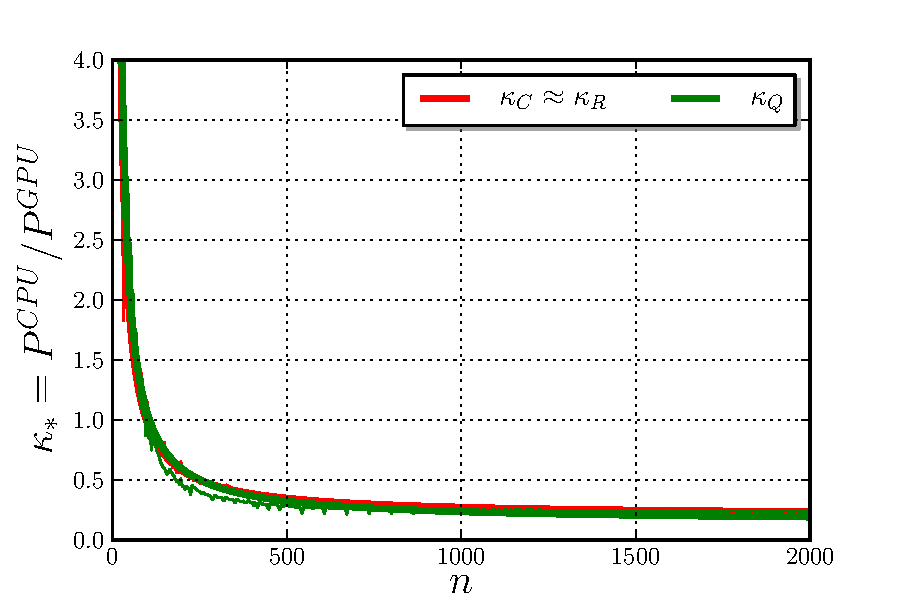
\includegraphics[width=\textwidth]{./figs/pdf/kappa_params}}
      
      %% Approximation approach
      \begin{itemize}
        \small
      \item 1st order rational functions of $n$
      \item Gauss-Markov estimator
      \end{itemize}
    \end{column}

    \begin{column}[t]{0.5\textwidth}
      \centering
      Switching ($l_F$) and  correction parameters 
      ($c_i$, $c_j$, $c'_k$, and $c''_k$)
      \visible<2->{
        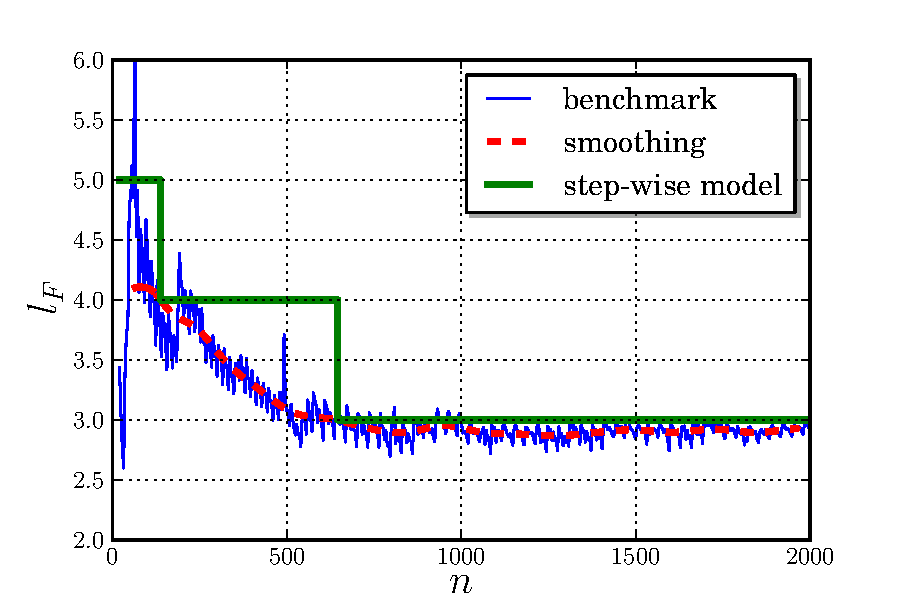
\includegraphics[width=\textwidth]{./figs/pdf/lF_param_approx}}

      %% Approximation approach
      \begin{itemize}
        \small
      \item %% descending 
        step-wise functions of $n$
      \item 1D filtering + rounding
      \end{itemize}
    \end{column}

  \end{columns}
\end{frame}

\begin{frame}{Experimental results}{Benchmarking results}
\begin{columns}[t]%[thb]
  \begin{column}[t]{0.5\textwidth}
    \centering
    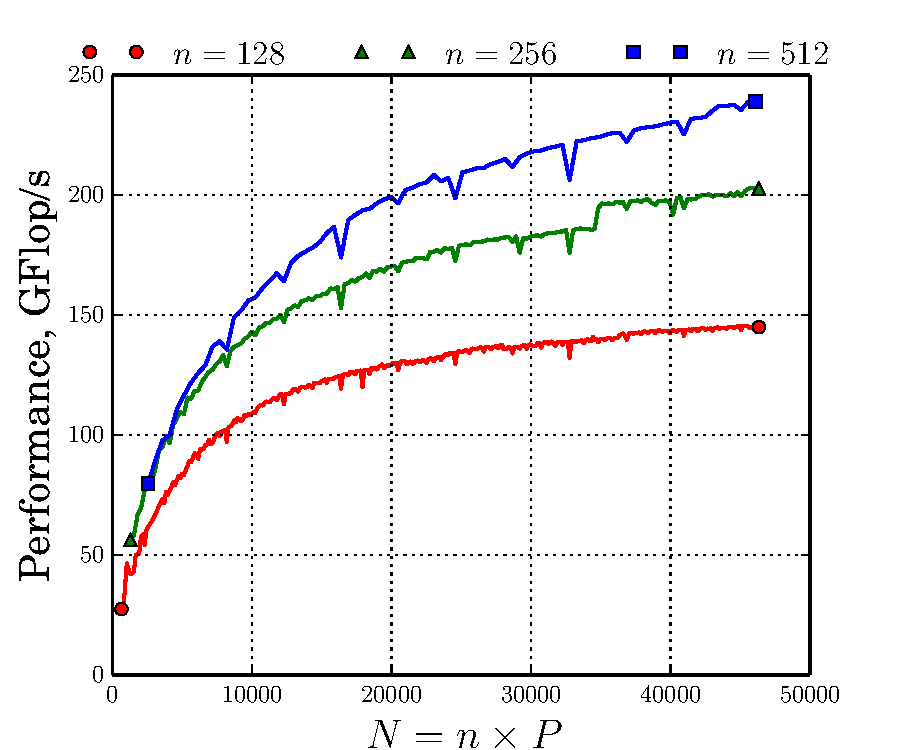
\includegraphics[width=\textwidth]{./figs/pdf/BSOFI_performance_scale}

    {Performance of the CPU, GPU and hybrid BSOFI codes}
  \end{column}
  \begin{column}[t]{0.5\textwidth}
    \centering
    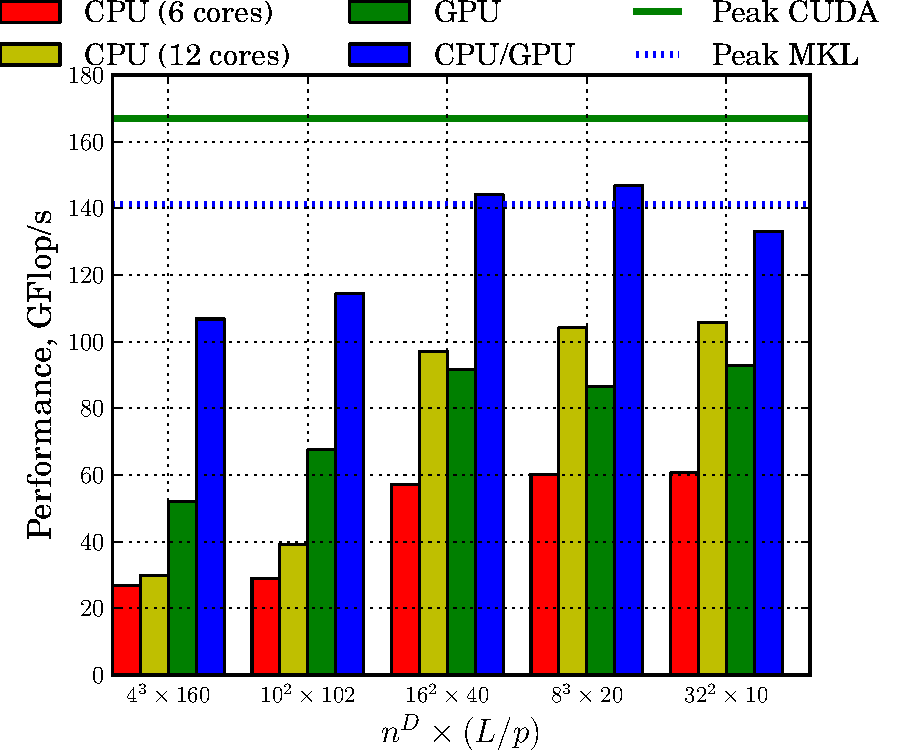
\includegraphics[width=\textwidth]{./figs/pdf/BSOFI_performance_sustainability}

    Performance of the hybrid BSOFI codes
  \end{column}
\end{columns}

\end{frame}

%% \frame[plain]{\centering
%%   \Huge Thank you for your attantion!

%%   \includegraphics[height=0.5\textheight]{figs/extras/question.jpg}
%% }

\end{document}
